\documentclass[tikz]{standalone}
\usepackage[outline]{contour}

\begin{document}
	    \contourlength{1.2pt}
\begin{tikzpicture}
    \node[anchor=south west,inner sep=0] at (0,0) {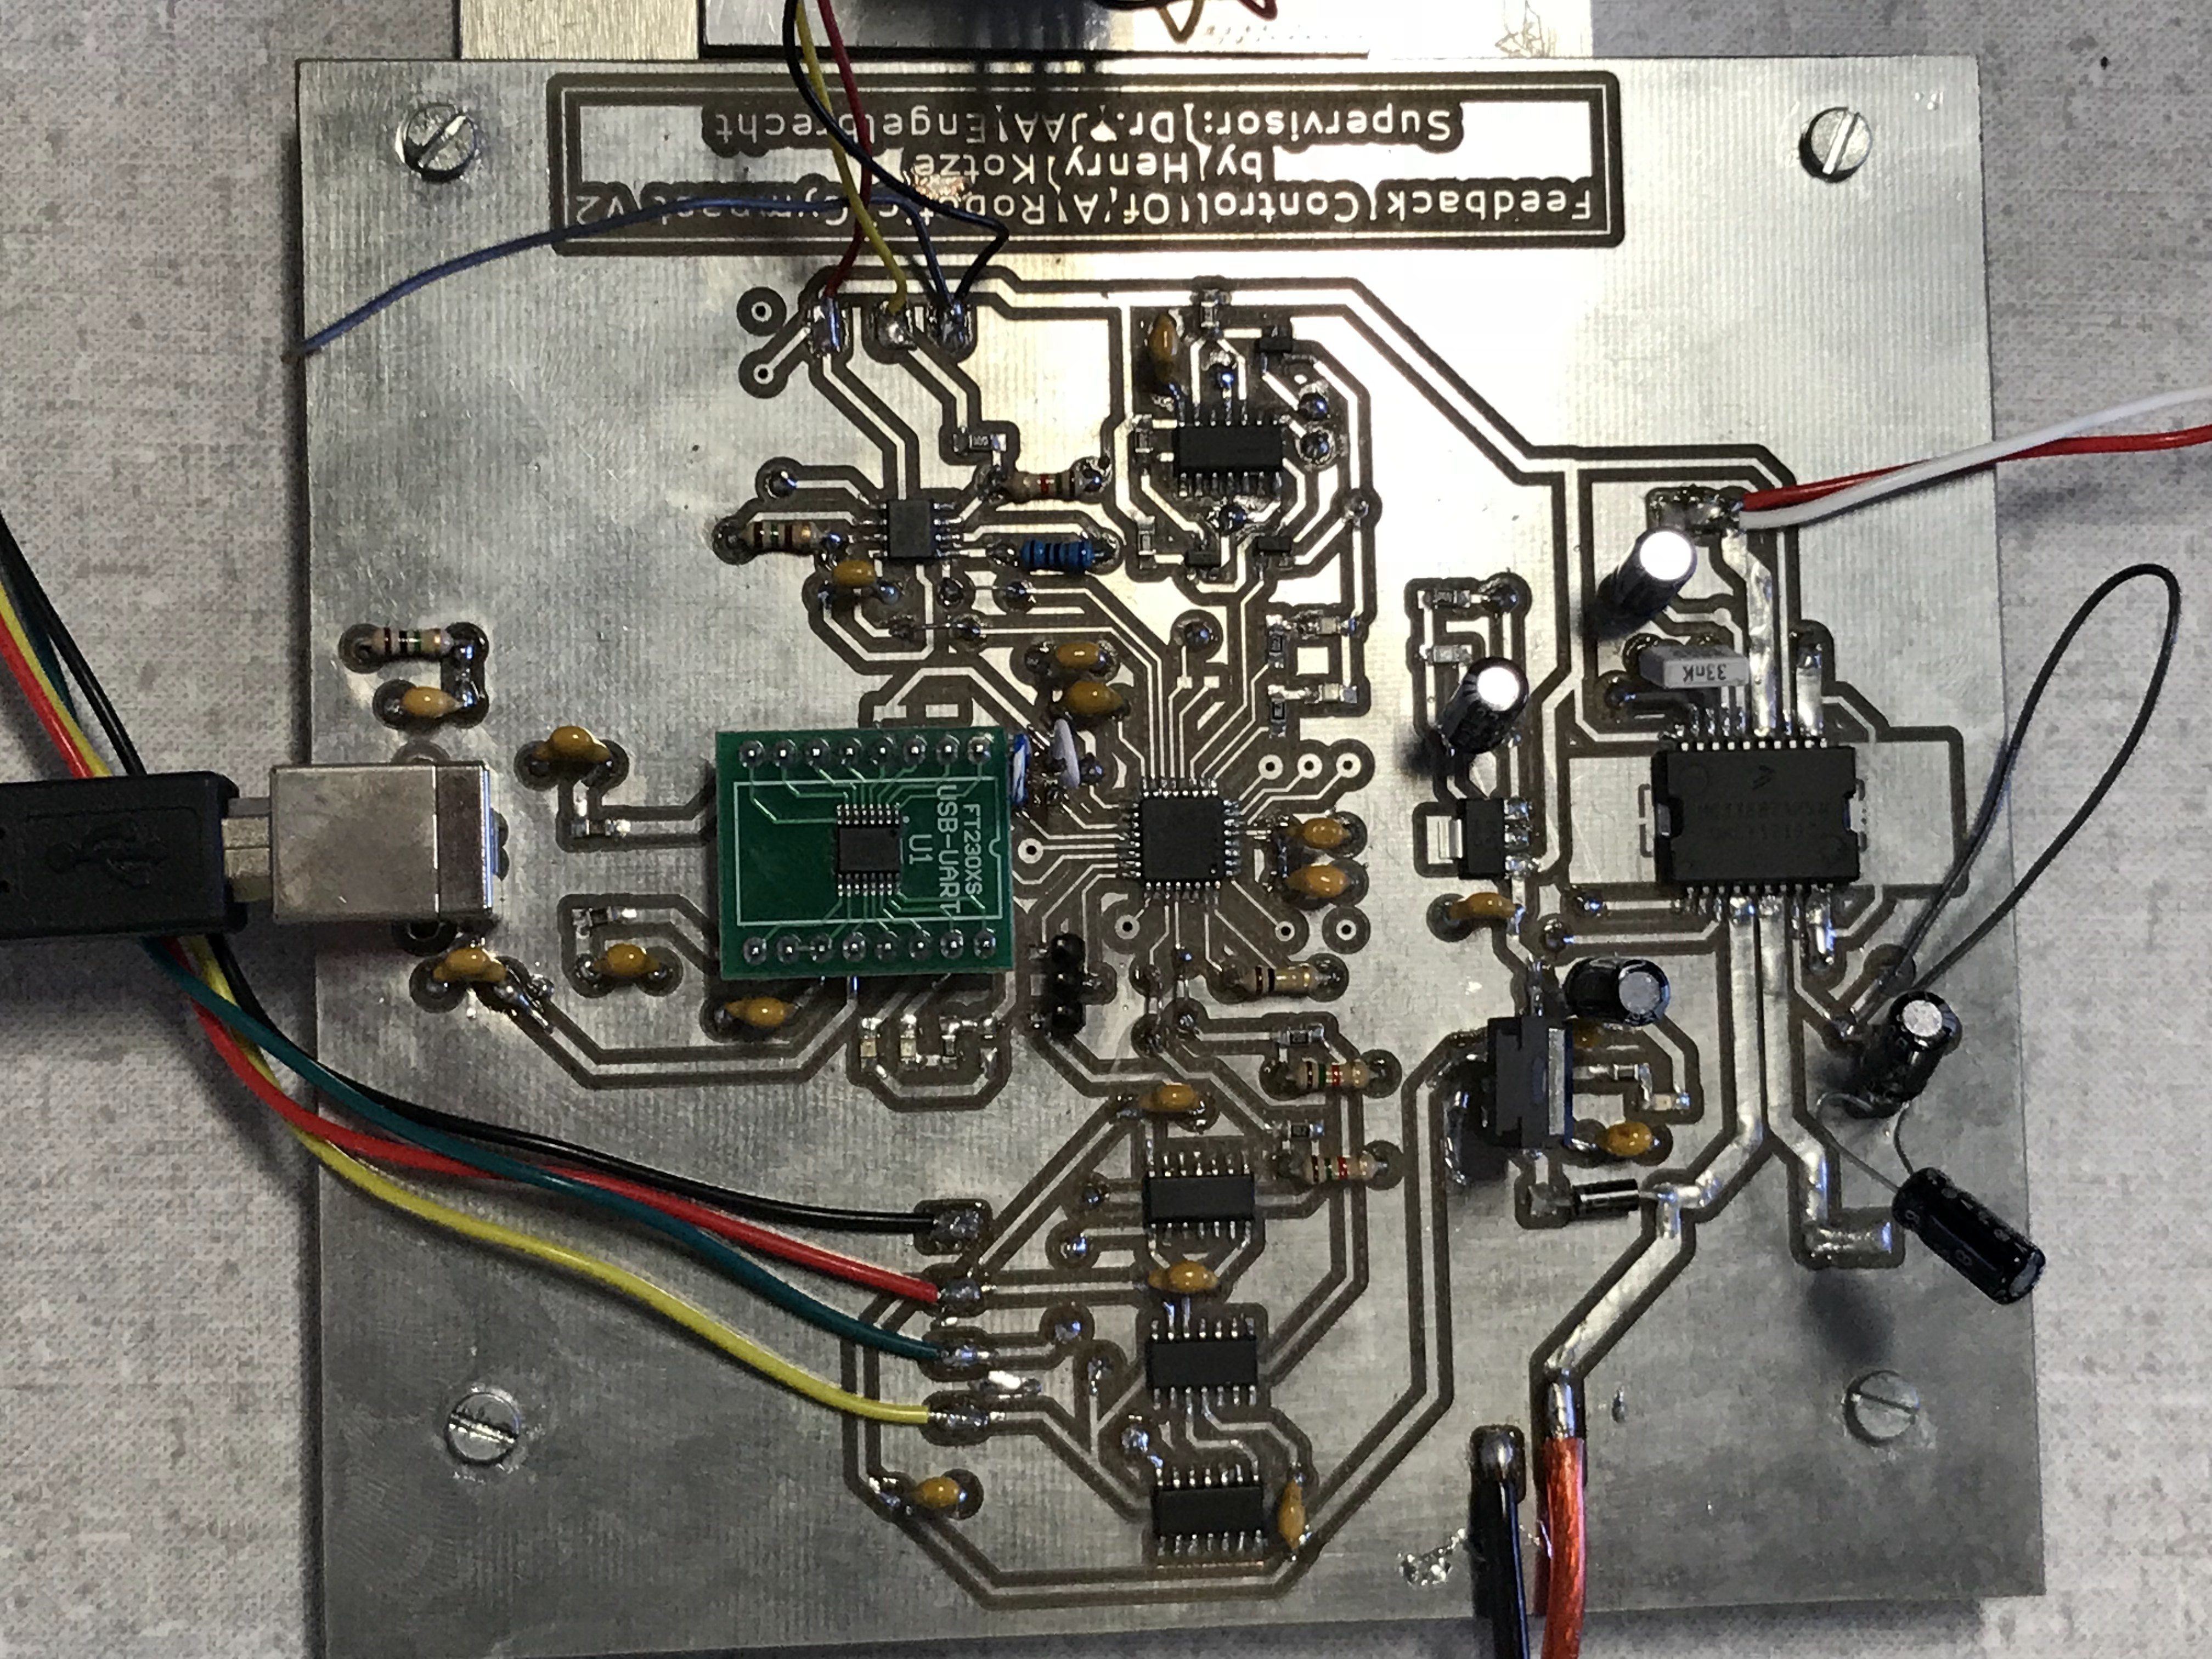
\includegraphics[width=\textwidth]{PCB.jpg}};
    %microcontroller
    %\draw[green,ultra thick,rounded corners] (6.5,5) node[above]{ \textbf{MCU} };
    

    
    \node[white] at (6.5,5.2) {\contour{black}{MCU}};
    
    \draw[red,ultra thick,rounded corners] (6,5) rectangle (7,4);
    
    %XOR
    \draw[red,ultra thick,rounded corners] (7.2,3) rectangle (6,0.5);
    \node[white] at (6.8,0.5) {\contour{black}{XOR, NOR Digital Circuit}};
    
    %UART
    \node[white] at (2.5,3.5) {\contour{black}{UART}};
    \draw[red,ultra thick,rounded corners] (1.5,3) rectangle (5.6,5.5);
    
    % AND
    \draw[red,ultra thick,rounded corners] (6,6) rectangle (7.5,7.5);
    \node[white] at (6.5,7.5) {\contour{black}{AND Digital Circuit}};
    
    %OPAMP
    \draw[red,ultra thick,rounded corners] (4,5.8) rectangle (5.5,6.5) ;
    \node[white] at (4.5,6.5) {\contour{black}{Op-Amp}};
    
    %REG
    \draw[red,ultra thick,rounded corners] (7.5,2.5) rectangle (8.8,6);
    \node[rotate=90,white] at (7.5,4.5) {\contour{black}{Regulators}};
    
    %Motor
    \draw[red,ultra thick,rounded corners] (9,2.5) rectangle (10.5,6);
    \node[rotate=90,white] at (10.5,4.5) {\contour{black}{Motor Driver}};
    
\end{tikzpicture}
\end{document}